\chapter{Plošina pro přistávání} \label{chap:pad}
  Rovné místo určené pro přistávání \acrshort{uav} s~vertikální dráhou přistávání se nazývá plošina pro přistávání, případně přistávací plošina nebo plocha. Může být pevná, přenosná či pohyblivá (s~vlastní lokomocí). Pevné plošiny jsou přímo spjaty s~místem jejich konstrukce, zatímco u~přenosných a pohyblivých lze měnit místo přistání. Obvykle se takto označují místa pro přistání malých letadel, plošiny pro větší stroje by se pak označily jako helipad nebo heliport.

  Všechna zmíněná místa většinou nesou nějaké vizuální označení, neboli fiducíární marker (\cref{sec:fidu}), které slouží k~jednodušší orientaci pilota, případně může podporovat autonomní přistání. Základní a nejpoužívanější variantou označení je velké písmeno H umístěné v~kružnici. V~oblasti autonomních \acrshort{uav} se plošiny často označují strojově čitelnou jedinečnou značkou, která nese i informaci, pomocí které se dá identifikovat.

  V~této práci byla použita plošina zkonstruovaná jako deska tloušťky 1{,}5~cm tvaru čtverce o~straně 70~cm. Celou plošinu vždy pokrýval rekurzivní fiduciární marker Apriltag o~2 vrstvách. Vnější vrstva o~rozměrech 10x10 buněk měla uprostřed díru o~rozměrech 2x2 buňky (rodina TagCustom48h12), do které byl umístěn tag vnitřní vrstvy o~rozměrech 8x8 buněk (rodina Tag36h11) obklopený bílou oddělovací čárou o~šířce 1 buňky vnitřního tagu. Rozměry značek jsou zde uvedeny včetně okraje, přičemž vnější značka měla jednu datovou vrstvu za okrajem.
  
  Plošina byla vždy umístěna vodorovně do terénu tak, aby ji ve svislém směru nic nezakrývalo a v~její blízkosti nebyly překážky, které by mohly přímo ovlivnit přistávání. Ve větší vzdálenosti mohla být umístěna překážka, která zastiňovala část plochy a tím i značky, čímž mohla být negativně ovlivněna přesnost a spolehlivost její detekce, což bylo prozkoumáno v~jednom z~experimentů (\refskl{sec:stin}{podkapitola}).
  \section{Fiduciární markery} \label{sec:fidu} %TODO: Doplnit obrázky tagů pro porovnání
    Fiduciární markery (nebo také značky) mohou mít mnoho podob (tvary, vzory, uspořádání klíčových prvků) a oblastí uplatnění (snímkování v~medicíně, mapování zemského povrchu, lokalizace zájmových bodů v~obrazu, v~robotice, identifikace jedinců atp.). Obecně se jako fiduciární marker označuje nějaký předmět, který slouží v~zorném poli zobrazovacího přístroje k~určení polohy daného zájmového bodu, jeho měřítka nebo jeho identifikaci. V~robotice se podle jejich obrazu zachyceného kamerou může určovat vzájemná poloha kamery a předmětu, na němž je značka připevněna.~\cite{kostak:fidmark}
    
    Možnosti určování vzájemné polohy se využívá v~této práci při odhadu umístění přistávací plošiny v~prostoru s~využitím kamery dronu. Dále budou uvedeny příklady některých používaných typů značek a popsány jejich základní vlastnosti. Pro hodnocení fiduciárních systémů, čili markerů a jejich detektorů, se používají metriky jako četnost falešných pozitiv, četnost záměny značky, četnost falešných negativ, minimální velikost značky \cite{artag}, doba trvání detekce \cite{aruco}; \cite{apriltag2} a další specifické vlastnosti. O~postupech používaných při detekci pojednává \cref{chap:detection}.
    \subsection{ARTag}
      ARTag je dvouodstínový fiduciární systém sestávající z~2002 značek, z~nichž polovina má černé okraje a polovina bílé. Prostor mezi okraji je vyplněn mřížkou o~rozměrech 6x6, přičemž každá z~buněk může být bílá nebo černá. Kromě kódovaných bitů obsahuje navíc i kontrolní součet, s~jehož využitím lze korigovat chyby (maximálně 2 bity z~36). Má nízkou četnost falešných pozitiv i četnost záměny značky za jinou. Ve srovnání se starším ARToolkit má vylepšenou identifikaci a verifikaci vzorů a snižuje tak četnost záměn značek. Přesto má větší knihovnu možných vzorů. \cite{artag}
    \subsection{Aruco}
      Fiduciární systém Aruco s~bity kódovanými pomocí čtverců nevyužívá předdefinovanou knihovnu vzorů, ale v~závislosti na požadavcích uživatele na velikost značky a slovníku generuje takové značky, které mají mezi sebou co nejvyšší vzdálenost, čímž se minimalizuje četnost záměn značek, a co největší počet přechodů mezi bity, čímž se minimalizuje četnost falešných pozitiv. Navíc je možné překrývat malé části značky a nenarušit tím detekci, nebo v~aplikaci využívat masku předmětu, kterým je tag zakryt, což je výhodné při využití pro rozšířenou realitu. \cite{aruco}
    \subsection{Apriltag}
      Dalším podobným systémem je Apriltag, který využívá podobné metody jako výše zmíněné systémy. Definuje různé typy, tzv. rodiny, značek v~závislosti na velikosti slova ve slovníku a minimální požadované Hammingovy vzdálenosti mezi tagy. I~v~tomto případě je tak možné zjišťovat a opravovat chyby při detekci značky. \cite{apriltag2}
      
      Ve verzi 3 je navíc dvakrát rychlejší detektor než ve verzi 2, umožňuje použití na míru navržených tvarů (např. kruhových nebo dokonce s~dírou) a data mohou být až za okrajem tagu, což zvyšuje datovou hustotu. Do prázdného místa uprostřed tagu je možné umístit další tag a vytvořit tak rekurzivní značku, kterou bude možné detekovat ve větším intervalu vzdáleností \cite{apriltag3}, toho bylo využito v~této práci jako značky na přistávací plošině (\cref{fig:customAprilTag}).

      \begin{figure}
        \centering
        \begin{subfigure}[b]{0.2\textwidth}
          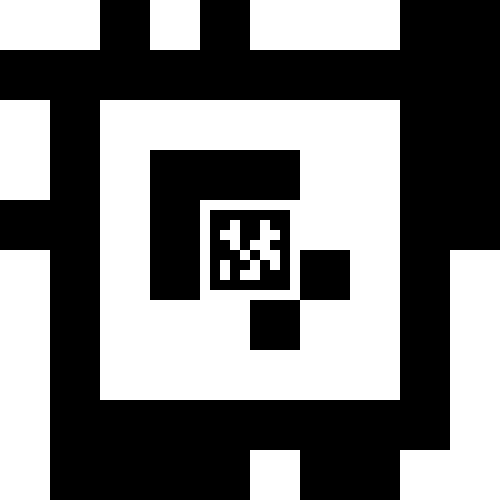
\includegraphics[width=\textwidth]{img/tag_48_12__36_11_164__137.png}
          \caption{Souosý dvouvrstvý AprilTag}
          \label{fig:customAprilTag}
        \end{subfigure}
        \caption{Příklady různých fiduciárních markerů}
        \label{fig:markery}
      \end{figure}
      